% Created 2016-04-09 Sa 09:51
\documentclass[presentation]{beamer}
\usepackage[utf8]{inputenc}
\usepackage[T1]{fontenc}
\usepackage{listings}
\usepackage{rotating}
\usepackage{amsthm,amsmath}
\lstset{
breaklines=false,
basicstyle=\ttfamily\footnotesize,
language=C++,
keywordstyle=\color{blue}
}


\usetheme{Goettingen}
\usecolortheme{beaver}
\author{}
\date{2016/04/12}
\title{Numerics}
\hypersetup{
 pdfauthor={Christian Kascha},
 pdftitle={Numerics},
 pdfkeywords={C++, Numerics, Programming},
 pdfsubject={Programming in C++},
 pdflang={English}}

\beamertemplatenavigationsymbolsempty


\begin{document}

\maketitle

%--------------------------------------------------------------- FOLIE
\begin{frame}{Outline}
\framesubtitle{}

\tableofcontents

\end{frame}
%--------------------------------------------------------------- 



\section{General}

%--------------------------------------------------------------- FOLIE
\begin{frame}{Floating Point Numbers}
\framesubtitle{}


\begin{itemize}
\item The computer has to save numbers such as $1/3 = 0.3333 \ldots$
  with a finite amount of memory.
\item Solution: floating point numbers:
  \begin{align*}
    (-1)^{s} \times (a_{1}.a_{2}a_{3}\ldots a_{t}) \times b^{e} &=
    (-1)^{s}\times m \times b^{e} \\ & \quad 1 \le a_{1} < b
  \end{align*}
\item Terms
  \begin{description}
  \item[$m$] mantissa
  \item[$t$] number of digits
  \item[$b$] basis
  \item[$e$] exponent
  \end{description}
\item Example: $3.3333 \times 10^{-1}$
\item Standard type in \texttt{C++}: \texttt{double}
\end{itemize}

\end{frame}
%--------------------------------------------------------------- 

%--------------------------------------------------------------- FOLIE
\begin{frame}{General implications}
\framesubtitle{}

\begin{itemize}
\item Only a finite range of numbers can be handled by a data type
\item Errors results when the range is left
  \begin{description}
  \item[Overflow] number is too high for a type
  \item[Underflow] number is too small for a type
  \end{description}
\item Numbers can only be stored approximately
\item Rounding errors result 
\end{itemize}

\end{frame}
%--------------------------------------------------------------- 

%--------------------------------------------------------------- FOLIE
\begin{frame}{Implications for $==$}
\framesubtitle{}

\begin{itemize}
\item Given a basis $b$ some numbers can be stored precisely, some not
  \begin{itemize}
  \item $1/2$ with $b=10$ and $3$ digits: $5.00 \times 10^{-1}$
  \item $1/3$ with $b=10$ and $3$ digits: $3.33 \times 10^{-1}$
  \end{itemize}
\item So ....
\lstinputlisting{prgs/round/main.cpp}
\end{itemize}


\end{frame}
%--------------------------------------------------------------- 


%--------------------------------------------------------------- FOLIE
\begin{frame}{Type Sizes in Bytes}
\framesubtitle{}

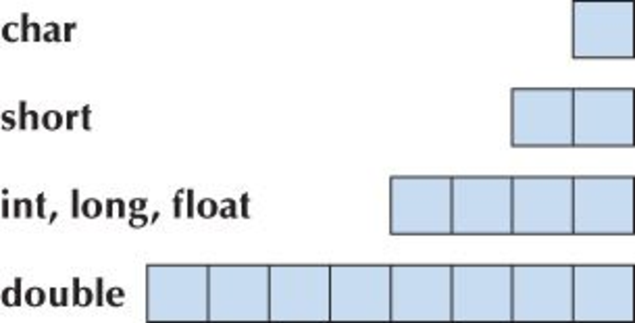
\includegraphics[scale=.5]{images/typesizes}

\begin{itemize}
\item When a \texttt{float} is assigned to an \texttt{int} digits get
  \textbf{truncated}: $3.14 \rightarrow 3$
\item When an \texttt{int} is assigned to a \texttt{float} you might
  loose \textbf{precision} when your \texttt{int} is too high $2100000009
  \rightarrow 2100000000$
\end{itemize}

\end{frame}
%--------------------------------------------------------------- 

%--------------------------------------------------------------- FOLIE
\begin{frame}{C++ Language Facilities}
\framesubtitle{}

\begin{itemize}
\item Header files: \texttt{<limits>, <climits>, <limits.h>, <float.h>}
\item \texttt{<limits>} gives \texttt{numeric\_limits<T>} for built-in types
  with member functions such as \texttt{min(), max(), lowest(), epsilon()} and
  many more \ldots 
\end{itemize}

\end{frame}
%--------------------------------------------------------------- 

%--------------------------------------------------------------- FOLIE
\begin{frame}{C++ Language Facilities}
\framesubtitle{}
\scalebox{0.8}{
\lstinputlisting{prgs/limits/main.cpp}
}
\end{frame}
%--------------------------------------------------------------- 


\section{The Matrix Library}

% --------------------------------------------------------------- FOLIE
\begin{frame}[fragile]{The Matrix Library}
  \framesubtitle{Why do we need one?}

  \begin{itemize}
  \item In principle we could use arrays.
  \item For example
\begin{lstlisting}
double my_matrix[3][4]; 
// declares a 3 x 4 matrix
\end{lstlisting}
  \item This is a bad idea.
  \end{itemize}

\end{frame}
% --------------------------------------------------------------- 


%--------------------------------------------------------------- FOLIE
\begin{frame}{The Matrix Library}
\framesubtitle{Access, Indexing}

\lstinputlisting{prgs/mataccess/main.cpp}

\end{frame}
%--------------------------------------------------------------- 

%--------------------------------------------------------------- FOLIE
\begin{frame}{The Matrix Library}
\framesubtitle{Dimensions}

\begin{itemize}
\item A matrix knows its dimensions.  
\end{itemize}
  \scalebox{0.8}{
    \lstinputlisting{prgs/matdim/main.cpp}}

\end{frame}
%--------------------------------------------------------------- 

%--------------------------------------------------------------- FOLIE
\begin{frame}{The Matrix Library}
\framesubtitle{Dimensions II}

\begin{itemize}
\item The dimensions are part of the matrix type. So you cannot write
  functions that take a general matrix. You would have to write a
  template for that.
\item Matrix is stored in memory in row-first fashion: 
\end{itemize}
  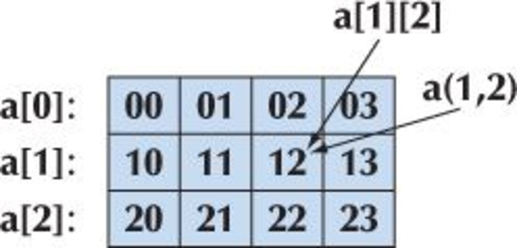
\includegraphics[scale=.5]{images/matrixidx} \vskip .5cm
  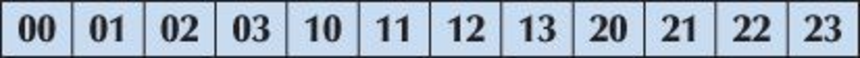
\includegraphics[scale=.5]{images/matrixelems}

\end{frame}
%--------------------------------------------------------------- 

%--------------------------------------------------------------- FOLIE
 \begin{frame}[fragile]{The Matrix Library}
   \framesubtitle{Slicing}

  \begin{itemize}
  \item Works with one-dimensional and two - dimensional matrices
  \end{itemize}
\begin{lstlisting}
 a.slice(i);    // the rows from the a(i) to the last
 a.slice(i,n);  // the rows from the a(i) to the a(i+n-1)
\end{lstlisting}

\end{frame}
%--------------------------------------------------------------- 


%--------------------------------------------------------------- FOLIE
\begin{frame}[fragile]{The Matrix Library}
\framesubtitle{Some common matrix functions}


\begin{lstlisting}
Matrix<int,2> a2 = a;  // copy initialization
a = a2;                // copy assignment
a *= 7;                // scaling (and +=, /=, etc.)
a.apply(f);            // a(i,j)=f(a(i,j)) for
                       //each element a(i,j)
a.apply(f,7);          // a(i,j)=f(a(i,j),7) for
                       // each element a(i,j)
b=apply(f,a);          // make a new Matrix with
                       // b(i,j)==f(a(i,j))
b=apply(f,a,7);        // make a new Matrix with
                       // b(i,j)==f(a(i,j),7)


a.swap_rows(1,2);      // swap rows a[1] <-> a[2]
\end{lstlisting}


\end{frame}
%--------------------------------------------------------------- 

%--------------------------------------------------------------- FOLIE
\begin{frame}{Matrix I/O}
\framesubtitle{}

\lstinputlisting{prgs/matio/main.cpp}

\end{frame}
%--------------------------------------------------------------- 

\section{Gaussian Elimination}

%--------------------------------------------------------------- FOLIE
\begin{frame}{Gaussian Elimination}
\framesubtitle{}

\begin{itemize}
\item Problem: Solve the linear system
  \begin{align*}
    A x = b 
  \end{align*}
  for $x$, where $A$ is quadratic ($n \times n$)
\item Solution: transform both sides of the equation such that $A^{*}$
  in 
  \begin{align*}
    A^{*} x = b^{*}
  \end{align*}
  is upper-triangular. 
\item Depending on the entries of $A^{*}$, the equation has zero, one
  or infinitely many solutions.
\end{itemize}

\end{frame}
%--------------------------------------------------------------- 

%--------------------------------------------------------------- FOLIE
\begin{frame}{Gaussian Elimination}
\framesubtitle{Solving the Upper-Triangular Form - Details}

\begin{itemize}
\item The system looks should like this at the end of the elimination
  \begin{figure}[h]
    \centering
    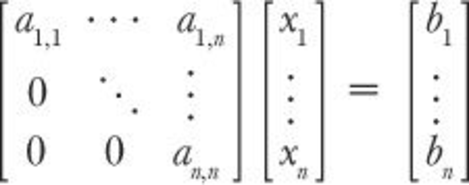
\includegraphics[scale=.5]{images/uppertriangularform}
  \end{figure}
\item Solve for $x[n] = b[n]/a(n,n)$, eliminate that row and solve for
  $x[n-1]$ and so on.
\item Works if all diagonal elements are non-zero, otherwise system
  has none or infinitely many solutions. 
\end{itemize}

\end{frame}
%--------------------------------------------------------------- 

\section{Random Numbers}

%--------------------------------------------------------------- FOLIE
\begin{frame}{Random Numbers}
\framesubtitle{}

\begin{itemize}
\item The sl header \texttt{<random>} has it.
\item Structure is
  \begin{description}
  \item[Engine] to generate uniformly distr. random integer(!) numbers
  \item[Distributions] map random numbers to distributions
  \end{description}
\end{itemize}

\end{frame}
%--------------------------------------------------------------- 



\section{Mathematical Functions \& Complex Numbers}

%--------------------------------------------------------------- FOLIE
\begin{frame}{Mathematical Functions \& Complex Numbers}
\framesubtitle{}

\begin{itemize}
\item Mathematical functions can be found in \texttt{<cmath>}. They
  have the usual names, that is, \texttt{cos, sin, floor} etc.
\item Complex numbers are in \texttt{<complex>}. 
\item For some weird reason, complex numbers are implemented as a
  template, so you have to initialize like 

\lstinputlisting{prgs/comp/main.cpp}
\end{itemize}


\end{frame}
%--------------------------------------------------------------- 

%--------------------------------------------------------------- FOLIE
\begin{frame}{The End}
\framesubtitle{}

\begin{center}
  Merci for listening.
\end{center}


\end{frame}
%--------------------------------------------------------------- 




\end{document}





